% !TeX root = ../main.tex

\chapter{国内外研究现状}

近年来深度神经网络算法在计算机视觉、自然语言处理等领域得到广泛地应用,但是神经网络模型庞大的模型大小和计算量使其难以在资源受限的设备上部署。这种矛盾在现阶段延缓了深度学习模型的大规模使用,因此轻量化网络设计成了学术界和商业界的研究热点。如图 \ref{fig:lightweight} 所示,轻量化网络实现方法分为网络结构设计\cite{mobilenet,squeezenet,shufflenet}和模型压缩两大类,其中模型压缩可以分为网络量化\cite{yan2020accurate,wang2020apq,cai2020zeroq}、模型剪枝\cite{han2015learning,he2017channel}、参数低秩分解\cite{denton2014exploiting,lebedev2016fast}、知识蒸馏\cite{hinton2015distilling,dai2021general,du2022distilling}等方法。在众多模型压缩方法中,网络量化是现阶段技术最成熟、应用最广泛的方法,目前已经可以实现不影响网络性能的条件下将32位浮点数运算转换为8位定点数运算。英伟达、寒武纪等人工智能芯片硬件厂商也都在板卡中集成了8位定点数运算单元,从硬件上支持网络量化算法。极致的量化是神经网络的二值化,受网络量化算法成功的影响,神经网络二值化算法也得到越来越多研究人员的关注。本文重点对如何通过提升二值网络特征表示能力增强二值神经网络性能进行研究。计算机视觉是神经网络应用最成功的领域之一,本文主要研究应用于计算机视觉的卷积神经网络的二值化。本章将对二值卷积神经网络概述和二值神经网络设计两方面进行介绍。

\begin{figure}[htb]
  \vspace{6pt}
  \centering
  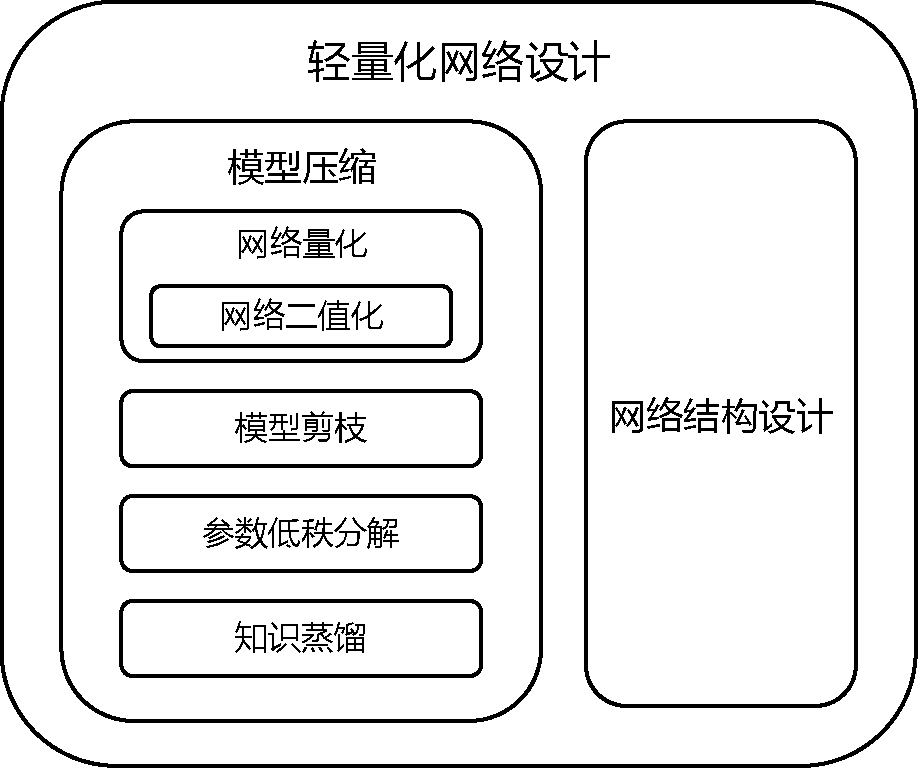
\includegraphics[width=0.7\textwidth]{lightweight.pdf}
  \caption{轻量化网络实现方法分类图}
  \label{fig:lightweight}
\end{figure}

\section{二值卷积神经网络概述}

卷积神经网络依赖其强大的归纳偏置广泛应用于图像识别、目标检测、语义分割、姿态估计等领域。对该类型神经网络进行二值化可以极大地解决其资源消耗过大的问题。本节先介绍传统卷积神经网络的组成和结构,然后介绍对卷积神经网络做二值化处理的通用方法。

\subsection{传统卷积神经网络}

由于图像的输入空间巨大,使用基于多层感知机的全连接神经网络处理图像任务会遇到网络过大、参数量过多的问题,导致网络无法在短时间内训练完成,即使完成训练也容易出现过拟合的现象。为了解决这个问题,早在1980年日本学者就提出了使用卷积模块构建神经网络用于图像分类任务\cite{fukushima1982neocognitron}。但当时没有受到更多的关注,直到2012年AlexNet\cite{alexnet}超过一众传统图像分类方法在ImageNet大规模视觉识别比赛中获胜,卷积神经网络的图像处理能力才获得关注,并最终广泛应用于基于神经网络的计算机视觉算法中。卷积神经网络一般由卷积层、池化层、归一化层、激活层、全连接层组成,其中卷积层是整个网络特征提取能力的核心,占全部计算量的90\%以上。针对卷积神经网络的各种结构设计和模型压缩方法也大部分是对卷积层的处理,因此本文先介绍图像的卷积操作,然后介绍卷积神经网络整体架构。

\subsubsection{图像卷积操作}

图像的卷积操作是对输入图像矩阵$\bm{x}$和权重矩阵$\bm{w}$做矩阵内积。其输入图像矩阵既可以是网络原始图像输入,也可以是网络中间的解析得到的特征矩阵即特征图。权重矩阵又称作卷积核或滤波器,在神经网络训练完成后其参数便固定不变。一般情况下特征图的尺寸较大,单方向元素个数有几十上百,而卷积核的尺寸较小,常见的尺寸有$3 \times 3$、$5 \times 5$、$7 \times 7$等。
% 卷积操作的实际计算如图所示(TODO),
计算图像卷积时,首先将卷积核放在特征图的左上角位置,然后卷积核和特征图上相同位置的元素相乘,所有相乘结果累加在一起作为输出矩阵左上角位置的值,然后将卷积核向右移动步长$S$的距离,进行上述相同的计算,得到输出矩阵第一行第二个位置的值,卷积核逐渐滑过整张特征图,计算出输出矩阵中全部的数值。

人们认为,卷积计算模式的两个特点使其能很好地处理图像任务。一是局部连接,卷积提取的是基于邻域的特征,邻域的大小就是卷积核的大小。局部连接避免了提取全局特征时连接量和计算量过大的缺点。虽然单层卷积的感受野只有卷积核大小,但是多层卷积堆叠可以线性扩大感受野,从而实现对全局的特征提取。二是卷积的权重共享性质,卷积核在特征图上滑过,特征图不同的区域使用同一个卷积核提取特征,这样做极大的减少了网络的参数量,避免了参数量过大导致的过拟合问题。同时,使用同一模式的卷积核在不同位置提取特征天然符合图像的平移不变性,有利于增强特征提取过程的鲁棒性。

\subsubsection{卷积神经网络架构}

现代卷积神经网络一般由卷积层、池化层、激活函数层、批归一化层、全连接层组成。卷积层使用上述图像卷积操作对特征图进行特征提取。池化层分为最大池化、平均池化等,主要用于调整减少图片的尺寸。激活函数层使用逐元素的非线性激活函数对输入进行处理,用于为网络提供非线性拟合能力,是卷积神经网络中必不可少的组成成分。批归一化层\cite{bn}是谷歌提出的用于调整网络中间层特征分布的网络层,几乎被后续所有卷积神经网络所使用。其定义如公式 \eqref{eq:bn} 所示:

\begin{equation}
  \label{eq:bn}
  y = \gamma \frac{x - \text{E}[x]}{\sqrt{\text{Var}[x]}} + \beta 
\end{equation}
其中$\gamma$和$\beta$是可学习参数,由网络训练得到。批归一化层可以将网络中间层归一化为有参数的正态分布,有效的避免了网络训练过程中的梯度爆炸或梯度消失,有利于训练很深的神经网络。全连接层在网络中起到分类器的作用,一般在网络最后使用1到2层。

几种不同网络层顺序堆叠形成网络模块,重复堆叠网络模块可得到整个网络结构。典型的用于图像分类的卷积神经网络结构如图 \ref{fig:cnn} 所示。其中softmax用于计算输出类别概率,该函数定义如公式 \eqref{eq:softmax} 所示:

\begin{equation}
  \label{eq:softmax}
  f(z_j) = \frac{\text{e}^{z_j}}{\sum_{i = 1}^{n} \text{e}^{z_i}} 
\end{equation}
其中$z_j$表示softmax层输入向量的第$j$个元素,$n$表示类别总数,通过softmax的归一化计算,可以抑制次要特征,凸显主要特征,决定分类概率。

\begin{figure}[htb]
  \vspace{6pt}
  \centering
  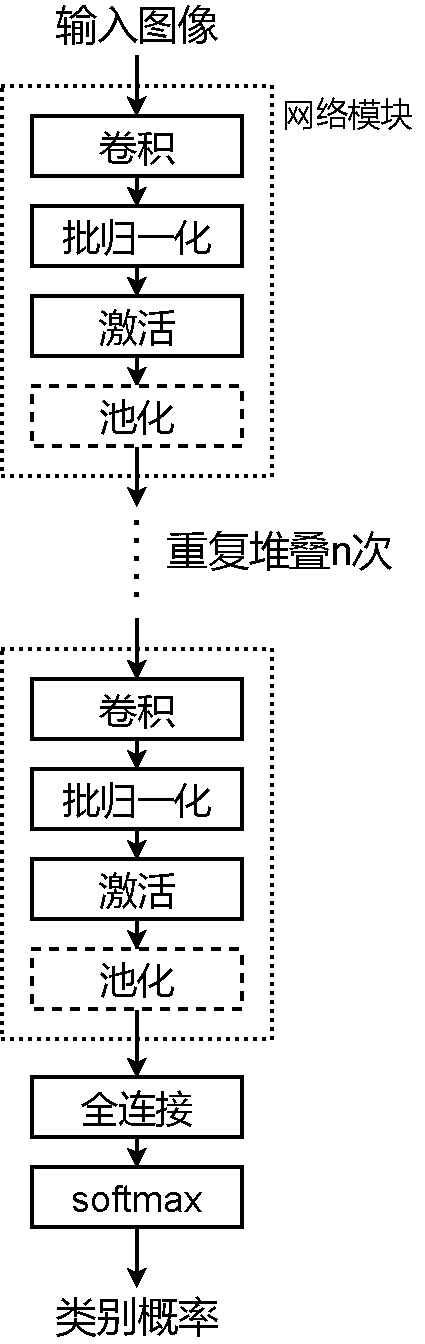
\includegraphics[width=0.3\textwidth]{cnn.pdf}
  \caption{用于图像分类的经典卷积神经网络结构图}
  \label{fig:cnn}
  \vspace{9pt}
\end{figure}

\subsection{神经网络二值化方法}

卷积神经网络主要依靠卷积层和激活函数层对特征进行提取。在全精度卷积神经网络中,提取特征的基本模块可以表示为:

\begin{equation}
  \bm{z} = \sigma (\bm{w} \otimes \bm{x})
\end{equation}
其中$\bm{x}$是激活值构成的特征张量,$\bm{x}$是权重张量,$\otimes$表示卷积操作,$\sigma(\cdot)$表示非线性函数,$\bm{z}$是输出张量。卷积操作中需要进行大量的乘法和加法操作,是卷积神经网络的性能瓶颈。为了降低网络计算量,提高推理速度,人们设计了神经网络二值化方法,下面从特征前向传递和梯度反向传播两方面介绍二值网络的实现方法。

\subsubsection{特征前向传递}

神经网络的二值化是对激活值和权重的二值化,使参与卷积计算的操作数都是1位表示。硬件上的1位只能表示两种状态,人们普遍使用$\{ -1, +1\}$作为二值取值,这是因为选取互为相反数的两值有利于激活值的均值稳定在0附近,如果选择$\{ 0, 1\}$作为二值取值,每次卷积的结果都一定是正数,激活值均值不稳定不利于网络的优化。激活值和权重的二值化过程可以表示为:

\begin{align}
  \bm{x}_b & = \phi_x(\bm{x}) \\
  \bm{w}_b & = \phi_w(\bm{w})
\end{align}
其中$\bm{x}_b \in \{ -1, +1\}$和$\bm{w}_b \in \{ -1, +1\}$分别是二值激活值张量和二值权重张量,函数$\phi(\cdot)$是一个逐元素二值函数。为了将浮点值映射到$\{ -1, +1\}$,普遍使用符号函数作为二值函数,如公式 \eqref{eq:sign} 所示:

\begin{equation}
  \label{eq:sign}
  \phi(x) = sign(x) =
  \begin{cases}
    -1 & if \ x < 0 \\
    +1 & if \ x \geq 0 
  \end{cases}
\end{equation}

经过二值化的特征提取基本模块可以表示为:

\begin{equation}
  \begin{split}
  \bm{z} & = \sigma (\phi_w(\bm{w}) \otimes \phi_x(\bm{x})) \\
  & = \sigma (\bm{w}_b \otimes \bm{x}_b)
  \end{split}
\end{equation}
可以看到卷积的输入都是二值数,卷积的本质是向量内积运算,二值向量内积在硬件上的实现方法如图 \ref{fig:bit} 所示,在硬件上用0表示-1,两个二值向量的逐元素乘法可以用同或位运算代替,二值向量元素的求和可以用位计数运算代替,将计数结果进行一定数学转换即可得到内积结果,二值向量计算过程可以表示为:

\begin{equation}
  \bm{x} \cdot \bm{y} = 2\ bitcount(xnor(\bm{x}, \bm{y})) - N
\end{equation}
其中$xnor$和$bitcount$分别是同或运算和位计数运算,位计数统计了向量中1出现的次数,$N$表示向量的元素个数。二值卷积中用位运算代替了浮点乘法和加法,在有专门硬件支持的情况下可以极大的提高运算速度。

\begin{figure}[htb]
  \vspace{6pt}
  \centering
  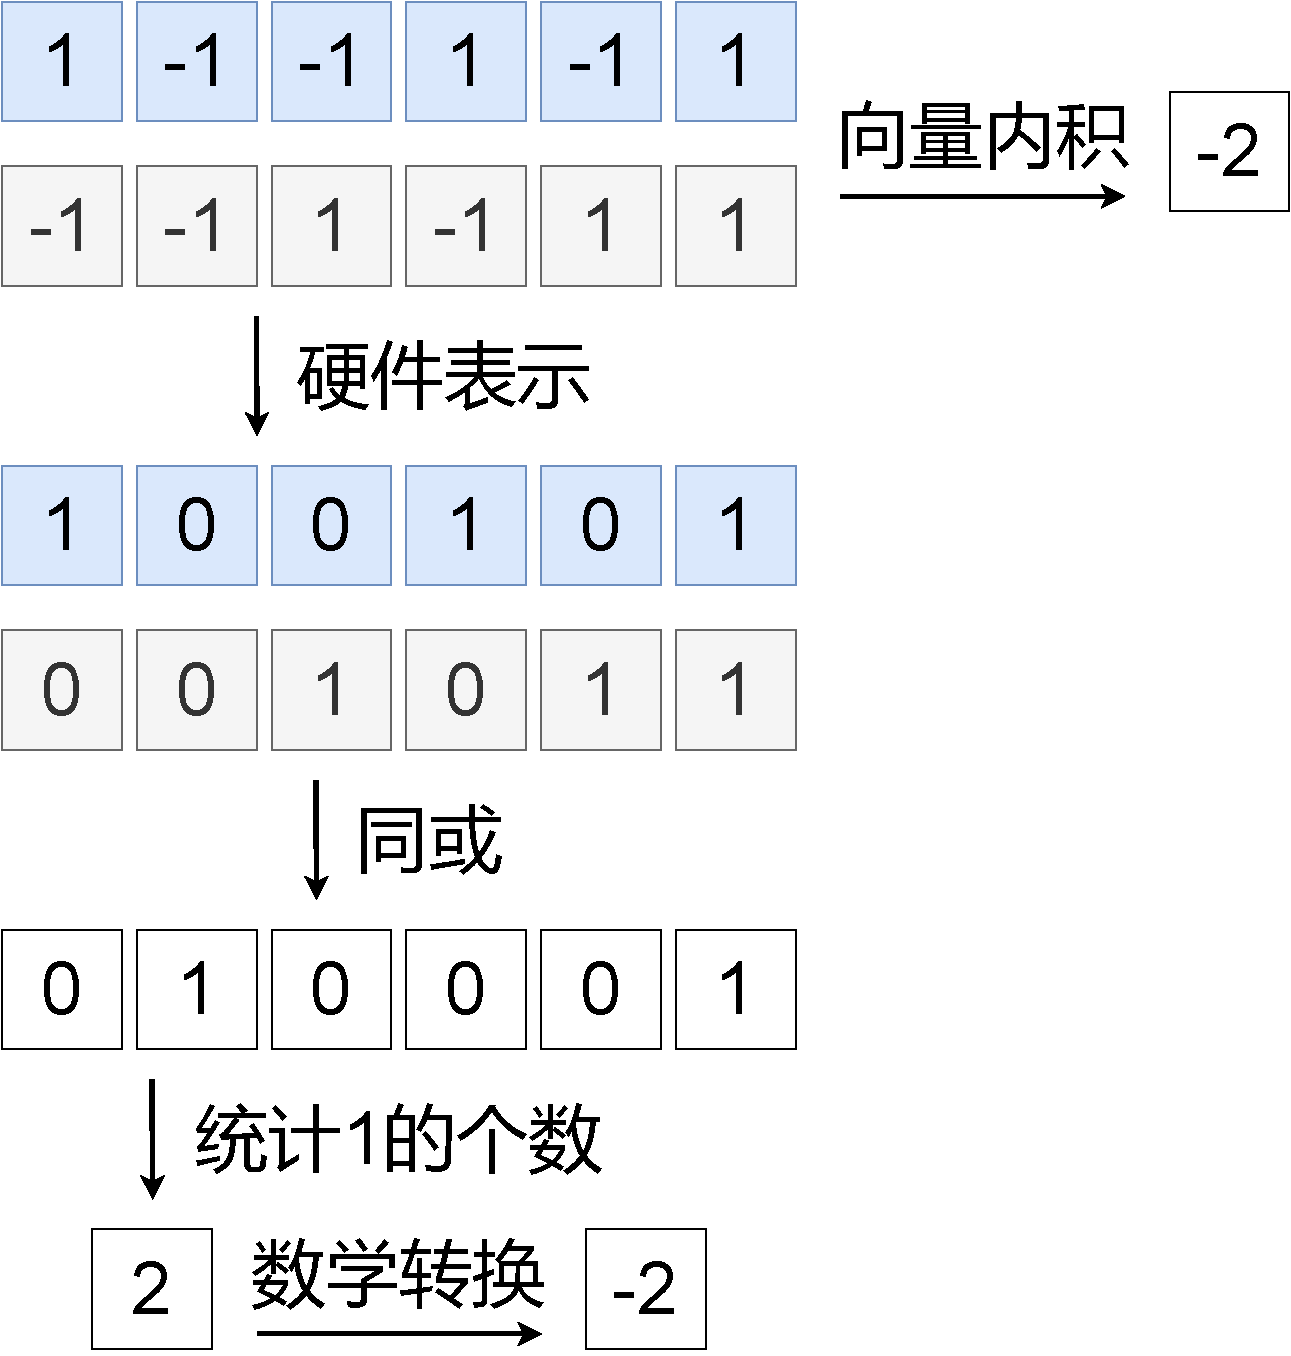
\includegraphics[width=0.5\textwidth]{bit.pdf}
  \caption{二值向量内积的硬件实现方法}
  \label{fig:bit}
  \vspace{6pt}
\end{figure}

\subsubsection{梯度反向传播}

神经网络使用梯度下降法对参数进行优化,二值神经网络同样使用这种方法训练,训练中需要计算浮点权重和浮点激活值相对于损失函数的梯度,根据链式法则其梯度可表示为:

\begin{align}
  \frac{\partial L}{\partial \bm{x}} & = \frac{\partial L}{\partial \bm{x}_b} \frac{\partial \bm{x}_b}{\partial \bm{x}} \\
  \frac{\partial L}{\partial \bm{w}} & = \frac{\partial L}{\partial \bm{w}_b} \frac{\partial \bm{w}_b}{\partial \bm{w}}
\end{align}
但是常作为二值函数的符号函数在原点外导数为0,造成梯度消失,浮点权重和浮点激活值的梯度始终为0,无法用梯度下降法更新参数。为了解决梯度传递问题,研究者在梯度反向传播的过程中使用直通估计器(STE)代替符号函数,截断函数$clip$是常用的直通估计器:

\begin{equation}
  \label{eq:clip}
  clip(x,-1,1) =
  \begin{cases}
    -1 & if \ x < -1 \\
    x & if \ -1 \leq x < 1 \\
    +1 & if \ x \geq 1
  \end{cases}
\end{equation}
可以看到,截断函数将输入的取值截断在$[-1, 1]$之间,当自变量取值范围为$(-1, 1)$时,该函数的导数为1,表示上游梯度和下游梯度相等,下游梯度可以忽略二值函数的存在向前传递。使用直通估计器时,前向传递和梯度反向传播使用的函数不同,会导致计算得到的梯度与真实梯度存在差异,这种现象称为梯度不匹配。研究表明\cite{xnornet},虽然二值网络的训练存在梯度不匹配,但是这仅造成二值网络训练的不充分,不影响训练的收敛。

\section{二值神经网络研究现状}

相同结构的二值网络性能明显差于浮点网络,较差的性能阻止了二值网络的实际应用。从二值网络的实现方法看,特征前向传递过程中的特征信息损失和梯度反向传播过程中的梯度不匹配是二值网络性能较差的两大原因。前向过程中32位浮点特征被二值函数提取为1位二值特征,特征表示能力大幅下降,同时二值函数的平滑和截断作用会引入大量噪声,使实际参与卷积运算的二值特征与浮点特征差异较大。反向过程中为了能够计算二值函数的梯度,引入了直通估计器在反向梯度计算时代替二值函数,这种替代造成的梯度差异会使网络整体优化方向出现偏差,导致二值神经网络难以训练。近几年,国内外学者针对二值神经网络存在的上述难点进行了大量研究,本文将所有研究概括为减小量化误差、优化梯度近似、提高训练能力、设计二值友好结构四个方向,下面对每个方向进行介绍。

\subsection{减小量化误差}

神经网络二值化是量化方法的一种极端情况,人们很自然的将网络量化中的概念和方法引入二值神经网络的研究。网络量化中的一个基本思路是减小量化误差,量化误差指权重或激活值在量化前后的差异,人们希望量化后的定点值与量化前的浮点值尽可能接近,从而使量化后的网络保持浮点网络的特征提取逻辑。在二值神经网络的研究中,很多研究者从量化误差的角度出发,设计方法使二值化后的二元值和二值化前的浮点值尽可能相近。由于二值化后取值过为单一,因此不可能要求输入张量二值化前后的逐元素相似性,只能计算整个张量的量化误差,使张量二值化前后从整体上更接近。

Rastegari等\cite{xnornet}最早将减小量化误差的思路引入神经网络二值化,并设计了BWN和XNOR-Net两种二值神经网络,其中BWN只对权重做二值化,激活值仍保持为浮点值,XNOR-Net则对权重和激活值都做二值化,该工作提出对每个需要二值化的参数增加缩放因子来减小二值化前后的量化误差,缩放因子$\alpha$通过最小化量化误差进行计算,如公式 \eqref{eq:xnornet} 所示:

\begin{equation}
  \label{eq:xnornet}
  \alpha^* = \mathop{\arg\min}\limits_{\alpha} ||\bm{w} - \alpha\bm{w}_b||^2
\end{equation}
根据最小化量化误差的要求,可以从激活值或权重的统计信息直接计算缩放因子。引入浮点缩放因子可以使二值神经网络的性能得到大幅提升,因此缩放因子被后续大部分研究所采用。Bulat等提出XNOR-Net++\cite{xnornet++},将权重和激活值的缩放因子融合为一个参数,并将该缩放因子作为可学习参数随网络一同优化,使缩放因子可以根据训练数据集自适应调节,无需在推理过程中动态计算,取得了比XNOR-Net更好的效果。在使用哈希映射训练二值权重网络\cite{bwnh}(BWNH)的工作中,研究者将权重二值化过程看作哈希映射过程,并引入可以减小量化误差的缩放因子帮助权重训练。Mishra等提出的大宽度低位宽网络\cite{wrpn}(WRPN)加大了网络的宽度,并用量化误差约束激活值的量化过程,在激活值和权重只有1位时仍维持了较好的性能。

ABC-Net\cite{abcnet}用加权组合多个二值基权重的结果近似原浮点权重,并通过最小化量化误差计算每个基权重的缩放因子,如公式所示:

\begin{equation}
  \label{eq:abcnet}
  \begin{split}
  \min_{\bm{\alpha}, \bm{w}_b}J(\bm{\alpha}, \bm{w}_b) & = ||\bm{w} - \bm{\alpha}\bm{w}_b||^2 \\
  & = ||\bm{w} - (\alpha_1 \bm{w}_{b1} + \alpha_2 \bm{w}_{b2} + \dots + \alpha_M \bm{w}_{bM})||^2
  \end{split}
\end{equation}
其中$M$表示基权重的数量,每个基权重都有各自的缩放因子,通过求解上述优化问题,可以尽可能使组合出的权重接近浮点权重,ABC-Net对激活值也进行同样的操作,在进行卷积计算时,需要根据乘法结合律将权重组合和激活值组合展开,保证卷积的输入是二元值,以便利用二值卷积的计算高效性,卷积计算策略如公式 \eqref{eq:abcnet_conv} 所示:

\begin{equation}
  \label{eq:abcnet_conv}
  \begin{split}
  conv(\bm{w}, \bm{x}) & \approx conv(\sum_{m = 1}^{M} \alpha_m \bm{w}_{bm}, \sum_{n = 1}^{N} \beta_n \bm{x}_{bn}) \\
  & = \sum_{m = 1}^{M} \sum_{n = 1}^{N} \alpha_m \beta_n conv(\bm{w}_{bm}, \bm{x}_{bn})
  \end{split}
\end{equation}
其中$N$表示作为组合的激活值个数,虽然该方法可以极大的减少量化误差,使二值网络的性能接近浮点网络,但是需要将原来的一个浮点卷积被拆分成$M \times N$个并行的二值卷积,增加了大量的计算量。

上述方法都是单独减小激活值或权重的量化误差,Wang等人\cite{tsq}指出单独考虑激活值或权重无法保证卷积的输出和浮点卷积输出相近,为了解决这个问题,Wang设计了两阶段训练方法,第一阶段保持权重为浮点值,使用量化函数$Q_a$将激活值量化到低位宽,第二阶段保持第一阶段得到的量化函数$Q_a$不变,基于量化误差优化低位宽$\bm{w}_b$权重和缩放因子$\alpha$,优化目标如公式 \eqref{eq:tsq} 所示:

\begin{equation}
  \label{eq:tsq}
  \min_{\alpha, \bm{w}_b} J(\alpha, \bm{w}_b) = ||\bm{z} - Q_a(\alpha(\bm{x} \otimes \bm{w}_b))||^2
\end{equation}
其中$z$表示原浮点卷积的结果,该工作使用迭代优化的思路对$\bm{w}_b$和$\alpha$进行优化,通过减小卷积输出的量化误差提升了网络量化或二值化后的性能。

\subsection{优化梯度近似}

二值神经网络使用梯度下降法进行训练,为了能计算二值函数的梯度,研究人员使用有梯度的直通估计器在反向传播过程中代替二值函数,常用的直通估计器如公式 \eqref{eq:clip} 所示,其前向函数和梯度函数图像如图 \ref{fig:clip} 所示。二值函数和直通估计器前向函数的不同导致了梯度不匹配问题,由于激活值二值化过程的梯度误差会在反向传播过程中不断累积,因此梯度不匹配会明显影响浅层网络的训练。为了缓解这个现象,研究人员设计了相比直通估计器更好的近似函数对符号函数的梯度进行近似。

\begin{figure}[htb]
  \vspace{6pt}
  \centering
  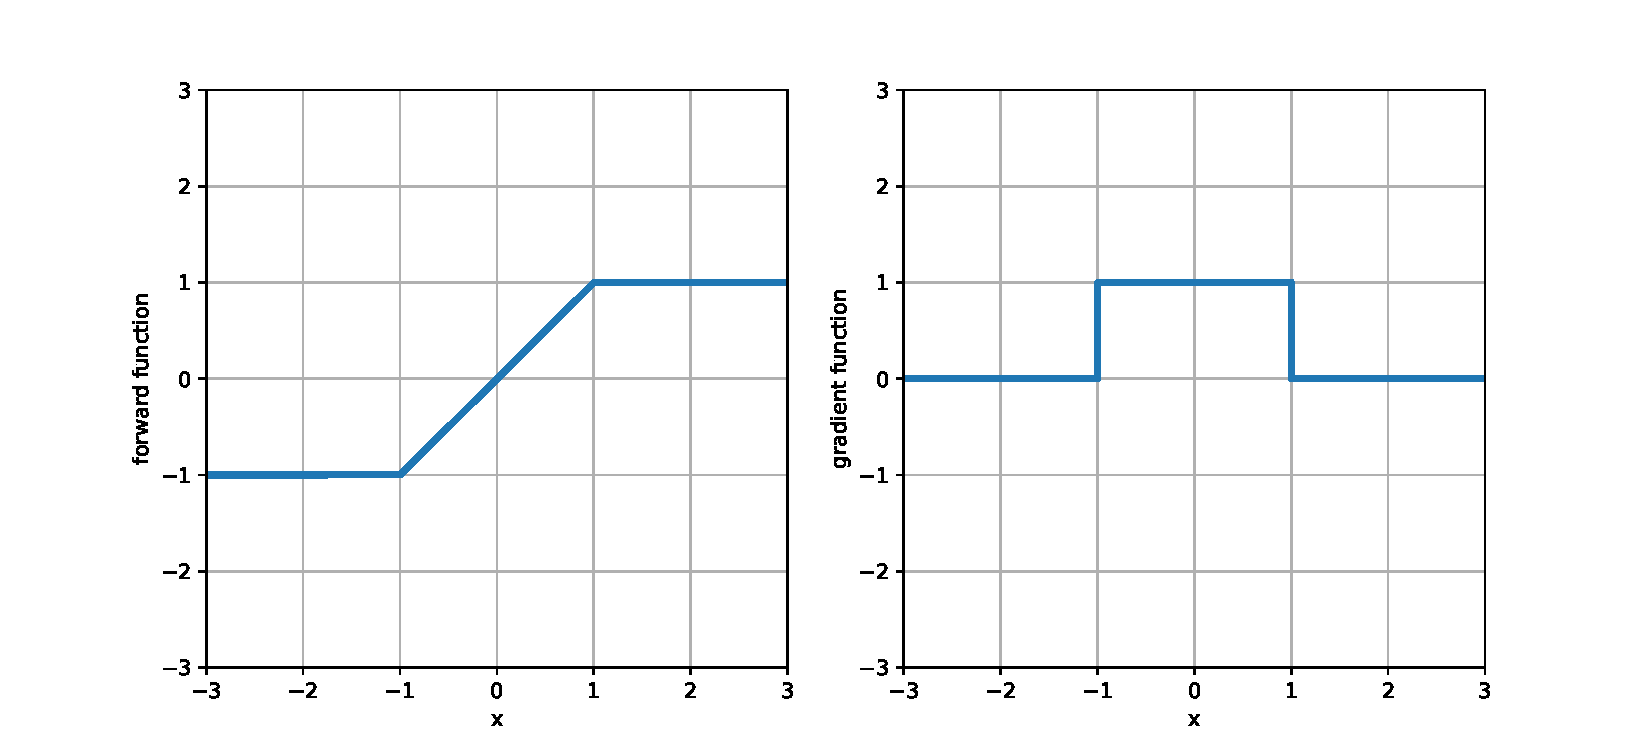
\includegraphics[width=0.9\textwidth]{ste1.pdf}
  \caption{截断近似函数的前向函数和梯度函数}
  \label{fig:clip}
\end{figure}

Bi-Real Net\cite{birealnet}中引入了一种二阶近似的直通估计器,使用分段二阶多项式函数近似符号函数,该估计器的前向函数如公式 \eqref{eq:ste_psign} 所示,反向函数如公式 \eqref{eq:ste_psign_d} 所示:

\begin{equation}
  \label{eq:ste_psign}
  psign(x) = 
  \begin{cases}
    -1 & if \ x < - 1 \\
    2x + x^2 & if \ - 1 \leq x < 0 \\
    2x - x^2 & if \ 0 \leq x < 1 \\
    +1 & if \ x \geq 1
  \end{cases}
\end{equation}

\begin{equation}
  \label{eq:ste_psign_d}
  \frac{\partial psign(x)}{\partial x} = 
  \begin{cases}
    2 + 2x & if \ - 1 \leq x < 0 \\
    2 - 2x & if \ 0 \leq x < 1 \\
    0 & \text{otherwise}
  \end{cases}
\end{equation}
二阶多项式近似的前向函数和梯度函数如图 \ref{fig:ste_psign} 所示,与截断函数相比,多项式近似函数的梯度值不是恒定的,而是随着自变量趋近于1或-1时趋近于0。实验表明使用多项式近似可以提高0.5\%左右的ImageNet分类精度。

\begin{figure}[htb]
  \centering
  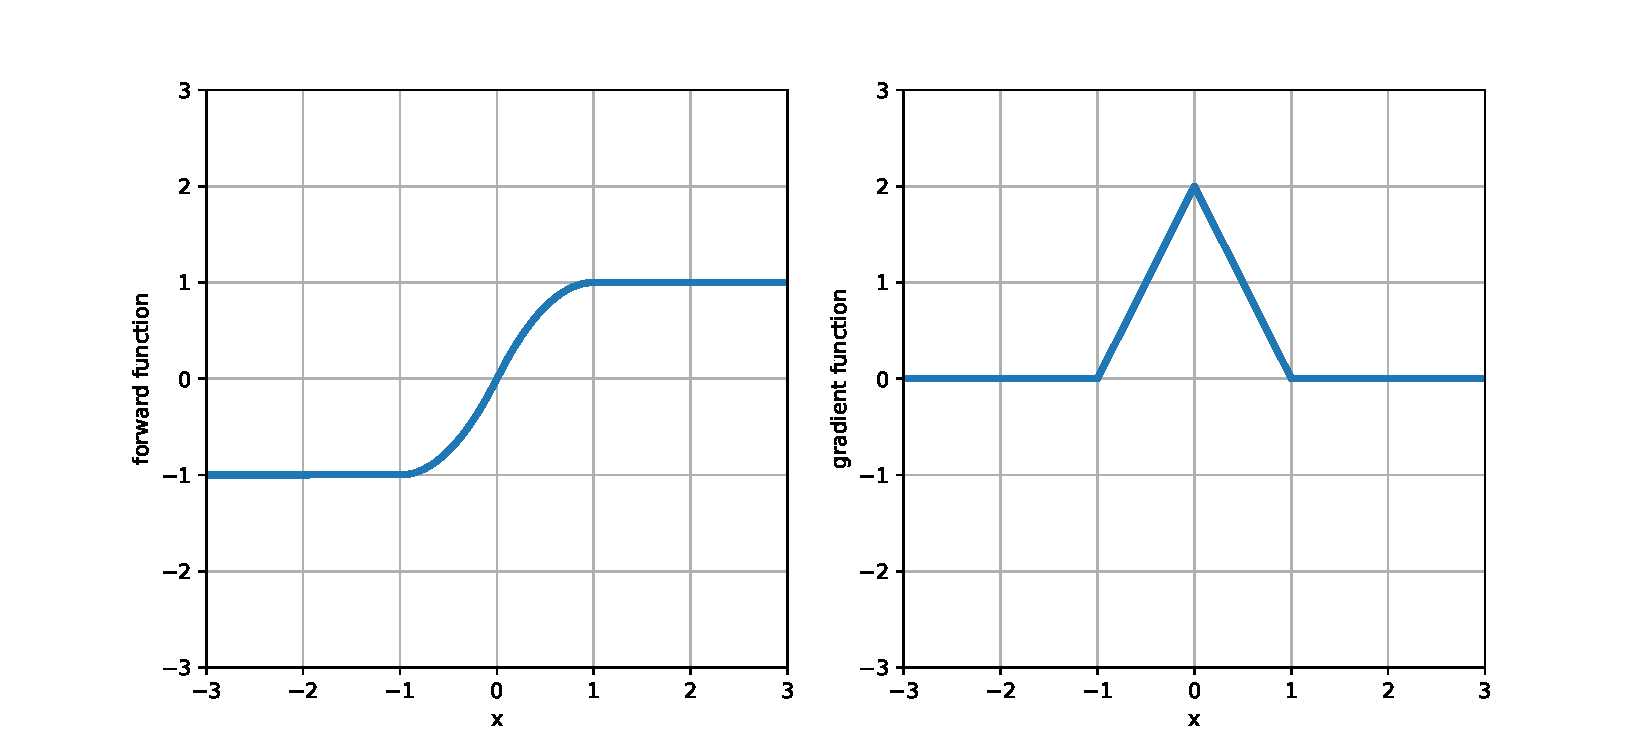
\includegraphics[width=0.9\textwidth]{ste2.pdf}
  \caption{多项式近似函数的前向函数和梯度函数}
  \label{fig:ste_psign}
\end{figure}

BNN+\cite{bnn+}参考了在神经网络中效果较好的Swish激活函数,设计了SwishSign函数作为符号函数反向传播的近似函数。SwishSign函数形式如公式 \eqref{eq:swishsign} 所示:

\begin{gather}
  \label{eq:swishsign}
  SwishSign_{\beta}(x) = 2\sigma(\beta x)(1 + \beta x(1 - \sigma(\beta x))) -1 \\
  \text{where} \quad \sigma (z) = \frac{1}{1 + e^{-x}} \notag
\end{gather}
其中$\beta > 0$是可变参数,用于控制近似函数在-1和1附近的变化速率,$\beta$可以作为网络的可学习参数进行优化。Swish近似函数的前向函数和反向函数如图 \ref{fig:swishsign} 所示。相比上述近似函数,Swish近似函数在-1和1附近仍有较大的梯度值,可以使浮点值在-1和1附近的激活值或权重得到较好的优化。

\begin{figure}[htb]
  \centering
  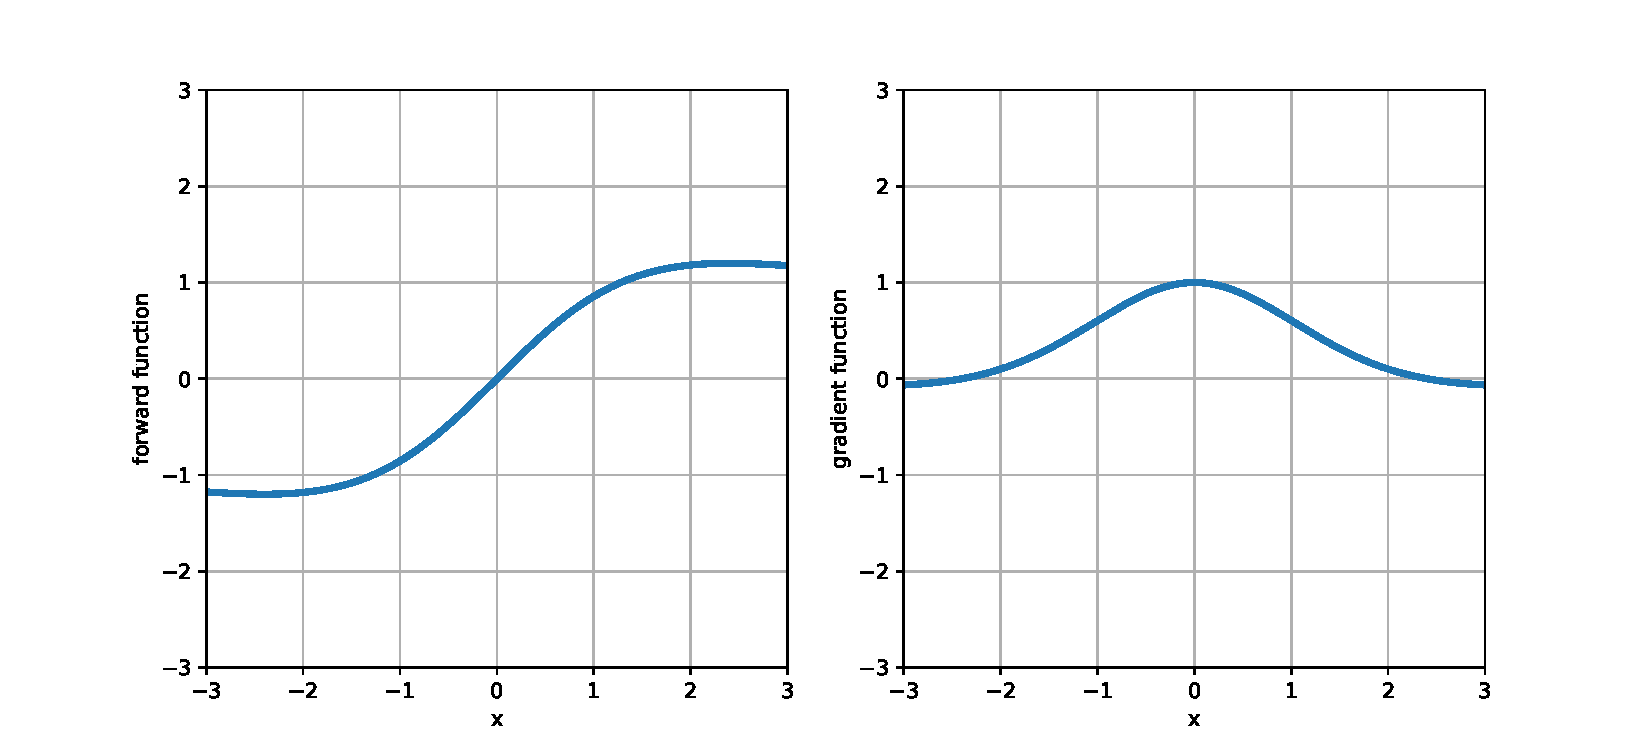
\includegraphics[width=0.9\textwidth]{ste3.pdf}
  \caption{$\beta = 3$时Swish近似函数的前向函数和梯度函数}
  \label{fig:swishsign}
\end{figure}

IR-Net\cite{irnet}提出二值函数的梯度近似函数应该考虑训练过程中需求的变化,设计了随着训练周期变化而变化的误差衰减近似器(EDE),该函数定义如公式 \eqref{eq:ede} 所示:

\begin{gather}
  \label{eq:ede}
  g(x) = k \tanh tx \\
  t = T_{min} 10^{\frac{i}{N} \times \log \frac{T_{max}}{T_{min}}} \notag \\
  k = \max(\frac{1}{t}, 1) \notag
\end{gather}
其中$g(x)$是EDE近似函数,$k$和$t$是随之网络训练变化的参数,$i$是训练的当前周期数,$N$是训练总周期数,$T_{min} = 10^{-1}$且$T_{max} = 10^{1}$,在训练初期,EDE近似函数具有较大的梯度值,有利于初期网络参数的更新,在训练后期,EDE近似函数仅在原点附近有梯度值,与真实的符号函数更加接近,有利于网络参数的微调优化。

\subsection{提高训练能力}

权重和激活值的二值化过程需要使用近似函数来传播梯度,固有的梯度不匹配现象会干扰二值神经网络的训练,导致训练不充分。很多研究从二值神经网络的训练角度入手,通过对训练过程的干预提高二值网络的训练能力。

设计额外的损失函数项可以指导训练时二值网络的学习方向。Hou等\cite{lab}认为现有二值网络的训练没有考虑二值化过程对损失函数的影响。他们提出基于对角海塞矩阵近似的拟牛顿算法,用来直接优化二值权重的损失函数,并通过实验验证了方法的有效性。Ding等\cite{ding2019regularizing}研究了二值神经网络中使用截断函数作为二值化反向近似函数导致的梯度流退化、饱和和不匹配现象,这些现象都会对二值网络的训练产生负面影响。为了改进训练过程,他们对激活值做正则化处理,通过限制激活值的分布消除二值网络训练中的不利情况。他们根据激活值的均值$\mu$和标准差$\sigma$分别设计了针对梯度退化的损失函数$L_D = [(|\mu|-k_{\epsilon}\sigma)_+)]^2$、针对梯度饱和的损失函数$L_S = [(k_{\epsilon}\sigma - 1)_+]^2$和针对梯度不匹配的损失函数$L_M = [(1 - |\mu| - k_{\epsilon}\sigma)_+]^2$,网络总损失函数可以表示为:

\begin{equation}
  L_{total} = L_{ce} + \lambda (L_D + L_S + L_M)
\end{equation}
其中$L_{ce}$是传统的交叉熵损失函数,$\lambda$是正则化损失函数的比例系数。他们的实验表明对激活值分布的约束可以有效提高二值网络的训练能力,从而在相同网络结构下提升分类任务上网络的精度。

Martinez等\cite{realtobin}认为二值卷积的输出特征和同结构浮点卷积的输出特征相近时,网络的性能会提高。为了在训练过程中引入浮点网络信息,他们提出了注意力损失函数,如公式 \eqref{eq:att} 所示:

\begin{equation}
  \label{eq:att}
  L_{att} = \sum_{j = 1}^{J} ||\frac{Q_S^j}{||Q_S^j||_2} - \frac{Q_T^j}{||Q_T^j||_2}||
\end{equation}
其中$J$是蒸馏点位个数,一般是4到5个,$Q^j$是特征图在通道维度上的均值,上标$S$表示二值网络,上标$T$表示相同结构的浮点网络。该注意力损失函数在二值网络的训练过程中引入了同结构浮点网络信息作为参考,实验表明这种额外信息的引入对二值网络训练有一定的帮助作用。ReActNet\cite{reactnet}中将浮点网络输出的分类评分作为软标签,二值网络本身的输出为硬标签,并在训练时使用软硬标签一同指导网络的优化。该方法从网络预测结果的角度为二值网络引入额外信息,有效提升了二值网络的训练能力。

\subsection{设计二值友好结构}

目前主流的网络量化算法将权重和激活值量化为8位定点数表示,8位数据的表示范围较大,量化前后的激活值和权重的数值分布不会发生较大改变,因此目前的量化方法多是通用量化方法,即可以应用于任何网络结构的量化方法。二值化将32位浮点数转换为1位表示,这种极致的信息压缩会显著改变权重和激活值的分布,导致二值化后的神经网络特征解析方式与原浮点网络明显不同,实验表明相同结构的神经网络二值化前后精度差异远大于量化。由于二值化的特殊性质,很难设计通用的二值化方法,在不损失精度的条件下将浮点网络转换为二值网络。研究人员们考虑二值神经网络对特征前向传递和梯度反向传播的特殊需要,设计了一些专门用于二值网络的二值友好模块结构或网络结构,用以提高二值神经网络的性能。

Bi-real Net\cite{birealnet}分析了二值化过程中特征信息的损失,认为连续两个或以上的二值卷积中后续卷积的输入信息过低,因此提出为每个卷积模块加一条残差连接,将每个卷积模块的浮点特征传递到下一个卷积模块,这种结构调整不仅增强了浮点特征的传递,还改善了反向传播时连续两个激活值二值化操作带来的梯度误差累积现象,实验证明这种结构改变对提升二值网络性能十分有帮助,后续的二值神经网络设计基本都使用了这种残差连接。Martinez等\cite{realtobin}提出在二值卷积前插入一个通道缩放模块,并将该模块的输出结果与二值卷积结果相乘,这种操作在保持二值卷积的计算高效性的同时为特征解析引入了额外的浮点信息,以极低的计算量为代价提高网络特征解析能力。Bulat等\cite{expert}从特征解析能力和模型拟合能力两方面对二值网络结构进行改进,对于特征解析能力,Bulat等设计了具有多个卷积核的专家二值卷积,对于不同的输入使用门函数选择不同的卷积核进行特征解析,弥补了单一二值卷积核解析能力不足的缺陷。对于模型拟合能力,Bulat等提出增加二值网络的宽度提高整体网络拟合能力,并将二值卷积改为分组二值卷积以保证计算量的不变,这些设计都有效的增强了二值网络的性能。MeliusNet\cite{meliusnet}通过增加通道数增加二值网络的特征表示能力,并使用额外残差连接对增加的通道信息进行整合,从而提高网络整体表示能力。

\section{本章小结}

本章介绍了二值神经网络的基本概念,详细介绍了二值网络前向传递和反向传播的实现方法。随后从减小量化误差、优化梯度近似、提高训练能力、设计二值友好结构四个方面介绍了二值神经网络的研究现状。减少量化误差是研究网络量化问题的重要方法,特别适合16位或8位量化。本文认为单纯减小量化误差不能有效降低二值网络特征在二值化过程的信息损失。本文认为二值特征的好坏在于是否从浮点特征中保留了有效信息,为此本文研究了如何从有效信息保留的角度提升二值网络的能力。现有的面向二值网络的结构设计没有充分发掘浮点计算在二值网络中的作用,本文对二值网络中的浮点计算进行了探究,设计了极低计算量的适合二值网络的浮点计算模块,有效提高二值网络性能。